\documentclass[11pt, a4paper]{report}
\usepackage[left=2.5cm,top=2.5cm,bottom=2.5cm,right=2.5cm]{geometry}
\usepackage{graphicx}
\usepackage{amsmath}
\usepackage{amssymb}
\usepackage{booktabs}
\usepackage{tikz}
\usetikzlibrary{shapes, arrows.meta, positioning, calc}
\usepackage{subcaption}
\usepackage{float}

\usepackage{titlesec}
\titleformat{\chapter}{\normalfont\huge\bfseries}{\thechapter.}{1em}{}
\titlespacing*{\chapter}{0pt}{-20pt}{20pt}

\usepackage[colorlinks=true, linkcolor=blue, urlcolor=blue, citecolor=blue]{hyperref}

\begin{document}

\chapter{Interference Graph Prediction with Edge-Aware GNNs}

\section{Introduction}
Constructing an accurate interference graph is fundamental for optimizing wireless networks. Traditional approaches often rely on precise physical location data and complex electromagnetic propagation models, which are often unavailable or impractical to maintain in dynamic environments. We propose an \textbf{Edge-Aware Graph Neural Network (GNN)} that infers the true interference graph solely from available AP telemetry and statistics, without requiring any knowledge of the physical AP locations. This approach enables robust interference estimation even in scenarios where physical topology is unknown or changing.

\section{System Model \& Inputs}
We model the wireless network as a graph $G=(V, E)$, where nodes $V$ represent APs and edges $E$ represent potential interference.

\subsection{Input Features}
Each AP is characterized by a feature vector $\mathbf{x}_i \in \mathbb{R}^{11}$. Recent updates have refined the energy features to be channel-specific. The features are:

\begin{itemize}
    \item \textbf{RF Environment (3)}: Incident Energy on Channel 1, 6, and 11 ($E_{ch1}, E_{ch6}, E_{ch11}$).
    \item \textbf{Traffic Load (2)}: Total Allocated Throughput ($T_i$), Number of Connected Clients ($C_i$).
    \item \textbf{Operational State (2)}: Duty Cycle ($D_i$), Transmit Power ($P_i$).
    \item \textbf{Mobility Dynamics (2)}: Roaming In Events ($R^{in}_i$), Roaming Out Events ($R^{out}_i$).
    \item \textbf{Configuration (2)}: Operating Channel ($Ch_i$), Bandwidth ($BW_i$).
\end{itemize}

\begin{figure}[H]
    \centering
    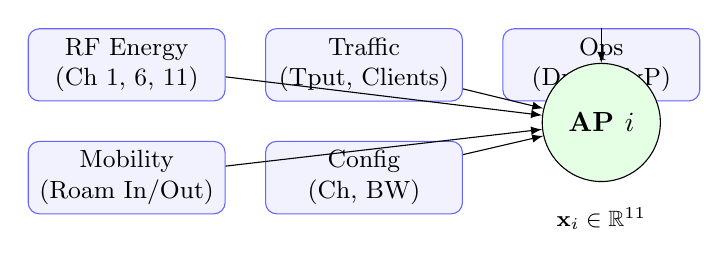
\begin{tikzpicture}[
        node distance=1.5cm,
        feature/.style={rectangle, draw=blue!60, fill=blue!5, rounded corners, minimum height=0.8cm, minimum width=2.5cm, align=center, font=\small},
        group/.style={rectangle, draw=gray!40, dashed, inner sep=0.3cm, rounded corners}
    ]
        % Feature Groups
        \node[feature] (rf) {RF Energy\\(Ch 1, 6, 11)};
        \node[feature, right=0.5cm of rf] (traffic) {Traffic\\(Tput, Clients)};
        \node[feature, right=0.5cm of traffic] (ops) {Ops\\(Duty, TxP)};
        \node[feature, below=0.5cm of rf] (mob) {Mobility\\(Roam In/Out)};
        \node[feature, right=0.5cm of mob] (config) {Config\\(Ch, BW)};

        % AP Node
        \node[circle, draw=black, fill=green!10, minimum size=1.5cm, right=1.0cm of config, yshift=0.7cm] (ap) {\textbf{AP $i$}};
        
        % Connections
        \draw[-latex] (rf) -- (ap);
        \draw[-latex] (traffic) -- (ap);
        \draw[-latex] (ops) -- (ap);
        \draw[-latex] (mob) -- (ap);
        \draw[-latex] (config) -- (ap);
        
        \node[below=0.2cm of ap, font=\footnotesize] {$\mathbf{x}_i \in \mathbb{R}^{11}$};
    \end{tikzpicture}
    \caption{Input Feature Composition for each Access Point.}
    \label{fig:inputs}
\end{figure}

\section{Architecture}
The core of our approach is the \textbf{EdgeConv} operator, which dynamically learns edge features by aggregating local neighborhood information.

\subsection{EdgeConv Layer}
For each edge $(i, j)$, the layer computes:
\[ \mathbf{e}_{ij} = \text{MLP}(\mathbf{x}_i \, \| \, \mathbf{x}_j - \mathbf{x}_i) \]
This formulation captures both the global properties of node $i$ and the local difference relative to neighbor $j$, essential for determining directional interference.

\begin{figure}[H]
    \centering
    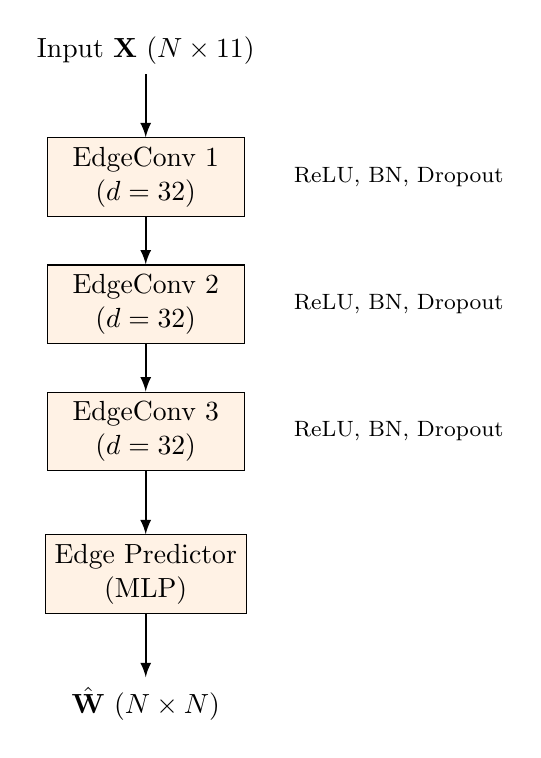
\begin{tikzpicture}[
        layer/.style={rectangle, draw=black, fill=orange!10, minimum width=2.5cm, minimum height=1cm, align=center},
        arrow/.style={-latex, thick}
    ]
        \node (input) {Input $\mathbf{X}$ ($N \times 11$)};
        \node[layer, below=0.8cm of input] (l1) {EdgeConv 1\\($d=32$)};
        \node[layer, below=0.6cm of l1] (l2) {EdgeConv 2\\($d=32$)};
        \node[layer, below=0.6cm of l2] (l3) {EdgeConv 3\\($d=32$)};
        \node[layer, below=0.8cm of l3] (pred) {Edge Predictor\\(MLP)};
        \node[below=0.8cm of pred] (output) {$\hat{\mathbf{W}}$ ($N \times N$)};

        \draw[arrow] (input) -- (l1);
        \draw[arrow] (l1) -- (l2);
        \draw[arrow] (l2) -- (l3);
        \draw[arrow] (l3) -- (pred);
        \draw[arrow] (pred) -- (output);
        
        \node[right=0.5cm of l1, font=\footnotesize, align=left] {ReLU, BN, Dropout};
        \node[right=0.5cm of l2, font=\footnotesize, align=left] {ReLU, BN, Dropout};
        \node[right=0.5cm of l3, font=\footnotesize, align=left] {ReLU, BN, Dropout};
    \end{tikzpicture}
    \caption{GNN Architecture: Stacked EdgeConv layers extract spatial dependencies to predict the interference matrix.}
    \label{fig:arch}
\end{figure}

\section{Experimental Results}
The model was trained on 1001 network snapshots (Train: 700, Val: 150, Test: 151) and evaluated on the held-out test set of 151 graphs.

\subsection{Performance Metrics}
\begin{table}[h]
    \centering
    \begin{tabular}{lcccc}
        \toprule
        \textbf{Metric} & \textbf{Value} & \textbf{Baseline (Mean)} & \textbf{Improvement} \\
        \midrule
        MAE & \textbf{0.0155} & 0.104 & 85.1\% \\
        RMSE & \textbf{0.0246} & 0.127 & 80.6\% \\
        $R^2$ & \textbf{0.986} & 0.000 & -- \\
        Pearson $r$ & \textbf{0.993} & -- & -- \\
        \bottomrule
    \end{tabular}
    \caption{Test set performance on diverse dataset (weights 0.0-0.7).}
\end{table}

\subsection{Visual Analysis}
The training curves (Fig. \ref{fig:training}) demonstrate rapid convergence. The prediction scatter plot (Fig. \ref{fig:scatter}) confirms the strong linear correlation between ground truth and predicted interference weights across the full range of interference conditions.

\begin{figure}[H]
    \centering
    \includegraphics[width=0.8\textwidth]{training_curves.png}
    \caption{Training dynamics showing loss convergence and $R^2$ improvement.}
    \label{fig:training}
\end{figure}

\begin{figure}[H]
    \centering
    \includegraphics[width=0.7\textwidth]{prediction_scatter.png}
    \caption{Scatter plot of Ground Truth vs. Predicted Interference Weights. The model maintains high accuracy ($R^2=0.986$) even with diverse interference conditions ranging from 0.0 to 0.7.}
    \label{fig:scatter}
\end{figure}

\section{Performance Analysis}
To validate the real-time feasibility of our approach, we profiled the system on a standard workstation. The profiling results, averaged over 100 simulation steps with 6 APs and 25 clients, are summarized in Table \ref{tab:performance}.

\begin{table}[h]
    \centering
    \begin{tabular}{lcc}
        \toprule
        \textbf{Operation} & \textbf{Mean Time (ms)} & \textbf{Std Dev (ms)} \\
        \midrule
        Physics Simulation Step & 2.16 & 0.78 \\
        GNN Data Preparation & 0.94 & 0.28 \\
        GNN Inference & 3.58 & 10.39 \\
        \textbf{Total Inference Pipeline} & \textbf{4.52} & \textbf{10.46} \\
        \bottomrule
    \end{tabular}
    \caption{Computational Performance Metrics. The total inference pipeline (Data Prep + Inference) takes approximately 4.5 ms, well within the requirements for real-time control loops (typically 10-100 ms).}
    \label{tab:performance}
\end{table}

In terms of resource usage, the system maintains a modest footprint, consuming approximately 340 MB of RAM and efficiently utilizing multi-core CPU resources (avg. 234\% usage) for parallelized tensor operations.

\section{Conclusion}
The proposed Edge-Aware GNN effectively approximates complex interference simulations. By leveraging 11 key RF and operational features, it provides accurate, real-time interference estimates, enabling dynamic and responsive wireless network management.

\end{document}